\documentclass[11pt]{article}
\usepackage{listings}
\usepackage{tikz}
\usepackage{enumerate}
\usetikzlibrary{arrows,automata,shapes}

\newtheorem{defn}{Definition}
\newtheorem{crit}{Criterion}

\newcommand{\handout}[5]{
  \noindent
  \begin{center}
  \framebox{
    \vbox{
      \hbox to 5.78in { {\bf Software Testing, Quality Assurance and Maintenance } \hfill #2 }
      \vspace{4mm}
      \hbox to 5.78in { {\Large \hfill #5  \hfill} }
      \vspace{2mm}
      \hbox to 5.78in { {\em #3 \hfill #4} }
    }
  }
  \end{center}
  \vspace*{4mm}
}

\newcommand{\lecture}[4]{\handout{#1}{#2}{#3}{#4}{Lecture #1}}
% 1-inch margins, from fullpage.sty by H.Partl, Version 2, Dec. 15, 1988.
\topmargin 0pt
\advance \topmargin by -\headheight
\advance \topmargin by -\headsep
\textheight 8.9in
\oddsidemargin 0pt
\evensidemargin \oddsidemargin
\marginparwidth 0.5in
\textwidth 6.5in

\parindent 0in
\parskip 1.5ex
%\renewcommand{\baselinestretch}{1.25}

\begin{document}

\lecture{11 --- January 30, 2019}{Winter 2019}{Patrick Lam}{version 0}

\section*{Review: Statements, branches and beyond}
We talked about statement (length-0 paths) and branch coverage
(length-1 paths) last time.  In lecture, we reviewed the elements
needed to satisfy these coverage criteria: given a graph and a
criterion, we get a set of Test Requirements $\mathrm{TR}$. We execute
each test $t$ in the test set $T$ on the system under test, giving a
set of test paths $p \in P$. The criterion is satisfied if there
exists at least one test path $p \in P$ that satisfies each of the
test requirements $\mathrm{tr} \in \mathrm{TR}$.

I'll say this again later, but for real programs, 80\% coverage is usually good enough; but
also consider what is not tested. Also, Assignment 1 Question 1 should point out to you that
it's possible to have 100\% statement coverage but not actually test anything, if you write
test cases that don't have asserts.

We could extend to paths of length 2 and beyond, but soon that gets us
to Complete Path Coverage (CPC), which requires an infinite number of
test requirements.

\begin{crit}
{\bf Complete Path Coverage}. (CPC) \emph{TR} contains all paths in $G$.
\end{crit}

Note that CPC is impossible to achieve for graphs with loops.

\section*{Testing State Behaviour of Software via FSMs}

We can also model the behaviour of software using a finite-state
machine. Such models are higher-level than the control-flow graphs that we've seen to date. They instead capture the design
of the software. There is generally no obvious mapping between a
design-level FSM and the code.

We propose the use of graph coverage criteria to test with FSMs.
\begin{itemize}
\item nodes: software states (e.g. sets of values for key variables);
\item edges: transitions between software states, i.e. something changes
in the environment or someone enters a command.
\end{itemize}
The FSM enables exploration of the software system's state space.  A
software state consists of values for (possibly abstract) program
variables, while a transition represents a change to these program
variables. Often transitions are guarded by preconditions and
postconditions; the preconditions must hold for the FSM to take the
corresponding transition, and the postconditions are guaranteed to
hold after the FSM has taken the transition.

\begin{itemize}
\item node coverage: visiting every FSM state = state coverage;
\item edge coverage: visiting every FSM transition = transition coverage;
\item edge-pair coverage (extension of edge coverage to paths of length at most 2): actually useful for FSMS; transition-pair, two-trip coverage.
\end{itemize}

\paragraph{Examples.} The next few graphs represent finite state machines
rather than control-flow graphs. Our motivation will be to set up
criteria that visit round trips in cyclic graphs.


\begin{center}
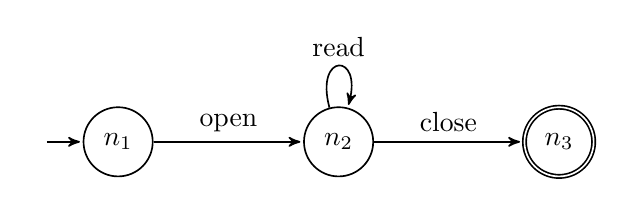
\begin{tikzpicture}[->,>=stealth',shorten >=1pt,auto,node distance=2.8cm,
                    semithick,initial text=]

  \node[initial,state]   (1)              {$n_1$};
  \node[state]           (2) [right of=1] {$n_2$};
  \node[accepting,state] (3) [right of=2] {$n_3$};
  
  \path (1) edge              node {open} (2)
        (2) edge              node {close} (3)
            edge [loop above]       node {read} (2);
\end{tikzpicture}
\end{center}
or perhaps
\begin{center}
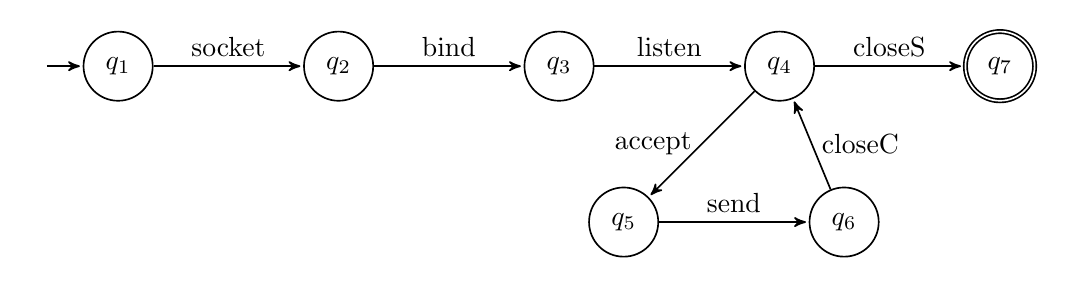
\begin{tikzpicture}[->,>=stealth',shorten >=1pt,auto,node distance=2.8cm,
                    semithick,initial text=]

  \node[initial,state]   (1)              {$q_1$};
  \node[state]           (2) [right of=1] {$q_2$};
  \node[state] (3) [right of=2] {$q_3$};
  \node[state] (4) [right of=3] {$q_4$};
  \node[state] (5) [below left of=4] {$q_5$};
  \node[state] (6) [right of=5] {$q_6$};
  \node[accepting,state] (7) [right of=4] {$q_7$};
  
  \path (1) edge              node {socket} (2)
        (2) edge              node {bind} (3)
        (3) edge              node {listen} (4)
        (4) edge              node {closeS} (7)
        (4) edge              node[left] {accept} (5)
        (5) edge              node {send} (6)
        (6) edge              node[right] {closeC} (4);
\end{tikzpicture}
\end{center}

The next criteria are mostly not for CFGs.
\begin{defn}
A \emph{round trip} path is a path of nonzero length with no internal cycles that starts
and ends at the same node.
\end{defn}

\begin{crit}
{\bf Simple Round Trip Coverage}. (SRTC) \emph{TR} contains at least one
round-trip path for each reachable node in $G$ that begins and ends a
round-trip path.
\end{crit}

\begin{crit}
{\bf Complete Round Trip Coverage}. (CRTC) \emph{TR} contains all round-trip
paths for each reachable node in $G$.
\end{crit}

\paragraph{Exercise.}  Create a Finite State Machine for some system that
you're familiar with.
%(In class, we saw a traffic light (AM) and for baking 
%cookies (PM); with the baking cookies example, we saw both an imperative
%FSM which is CFG-like and a more state-based FSM. We had a question about
%whether we could split the state-based FSM into an oven FSM and an
%ingrediate FSM. Yes, we could, but then we'd have to understand how
%to synchronize different FSMs, which is beyond the scope of this class.)

\subsection*{Deriving Finite-State Machines}
You might have to test software which doesn't come with a handy FSM.
Deriving an FSM aids your understanding of the software. (You might
be finding yourself re-deriving the same FSM as the software evolves;
design information tends to become stale.)

We'll see some tools---iComment and Daikon---for obtaining sequencing constraints from
comments/documentation and from the code.

%% Four techniques for deriving FSMs:
%% \begin{itemize}
%% \item use control-flow graphs;
%% \item use higher-level software structure;
%% \item model software's state variables; or
%% \item use specifications.
%% \end{itemize}

\paragraph{Control-Flow Graphs.} Does not really give FSMs.
\begin{itemize}
\item nodes aren't really states; they just abstract the program
counter;
\item inessential nondeterminism due e.g. to method calls;
\item can only build these when you have an implementation;
\item tend to be large and unwieldy.
\end{itemize}

\paragraph{Software Structure.} Better than CFGs.
\begin{itemize}
\item subjective (which is not necessarily bad);
\item requires lots of effort;
\item requires detailed design information and knowledge of system.
\end{itemize}

\paragraph{Modelling State.} 
This approach is more mechanical: once you've chosen relevant state
variables and abstracted them, you need not think much.

You can also remove impossible states from such an FSM, for instance
by using domain knowledge.

\paragraph{Specifications.}
These are similar to building FSMs based on software structure.
Generally cleaner and easier to understand. Should resemble UML
statecharts.

\paragraph{General Discussion.} Advantages of FSMs:
\begin{itemize}
\item enable creation of tests before implementation;
\item easier to analyze an FSM than the code.
\end{itemize}
Disadvantages:
\begin{itemize}
\item abstract models are not necessarily exhaustive;
\item subjective (so they could be poorly done);
\item FSM may not match the implementation.
\end{itemize}

\end{document}
